\documentclass[sigconf,9pt]{acmart}

%\usepackage[english]{babel}
%\usepackage{blindtext}
%\usepackage{listings}
\usepackage{tikz}

%\usepackage[compact]{titlesec}
%\newcommand{\newtodo}[1]{\textcolor{red}{#1}}

\newcommand{\pgftextcircled}[1]{
    \setbox0=\hbox{#1}%
    \dimen0\wd0%
    \divide\dimen0 by 2%
    \begin{tikzpicture}[baseline=(a.base)]%
        \useasboundingbox (-\the\dimen0,0pt) rectangle (\the\dimen0,1pt);
        \node[circle,draw,outer sep=0pt,inner sep=0.1ex] (a) {#1};
    \end{tikzpicture}
}

\usepackage{enumitem}
\setitemize{noitemsep,topsep=0pt,parsep=0pt,partopsep=0pt}
\setenumerate{noitemsep,topsep=0pt,parsep=0pt,partopsep=0pt}
\setdescription{itemsep=0pt,topsep=0pt,parsep=0pt,partopsep=0pt,itemindent=0em,leftmargin=0.5em}

% \us: "microseconds"
\newcommand{\us}{\textmu{}s\xspace}

%compressed environments
\newenvironment{denseitemize}{
\begin{itemize}[topsep=2pt, partopsep=0pt, leftmargin=1.5em]
  \setlength{\itemsep}{2pt}
  \setlength{\parskip}{0pt}
  \setlength{\parsep}{0pt}
}{\end{itemize}}

\newenvironment{denseenum}{
\begin{enumerate}[topsep=2pt, partopsep=0pt, leftmargin=1.5em]
  \setlength{\itemsep}{2pt}
  \setlength{\parskip}{0pt}
  \setlength{\parsep}{0pt}
}{\end{enumerate}}

\def\ie{{i.e.\ }}
\def\eg{{e.g.,\ }}
\def\etal{{et al.\xspace}}
\def\wrt{{w.r.t.\xspace}}
\def\etc{etc.\xspace}

\def\name{\texttt{cache\_ext}\xspace}

\newcommand{\tailpct}[0]{99\textsuperscript{th}-percentile}
\newcommand{\tailpctnnn}[0]{99.9\textsuperscript{th}-percentile}

\newcommand{\taillatency}[0]{\tailpct{} latency}
\newcommand{\taillatencynnn}[0]{\tailpctnnn{} latency}

\iftrue
\newcommand{\asaf}[1]{\textcolor{red}{\{Asaf: #1\}}}
\newcommand{\tal}[1]{\textcolor{red}{\{Tal: #1\}}}
\newcommand{\teng}[1]{\textcolor{red}{\{Teng: #1\}}}
\else
\newcommand{\asaf}[1]{}
\newcommand{\tal}[1]{}
\newcommand{\teng}[1]{}
\fi

\newcommand{\uffd}{\texttt{userfaultfd()}~}

\settopmatter{printacmref=false, printccs=false, printfolios=true}

%% {} with no args suppresses printing of the price
\acmPrice{}

\begin{document}

\acmYear{2024}
\copyrightyear{2024}
\setcopyright{rightsretained}
\acmConference[eBPF '24]{Workshop on eBPF and Kernel Extensions}{August 4--8, 2024}{Sydney, NSW, Australia}
\acmBooktitle{Workshop on eBPF and Kernel Extensions (eBPF '24), August 4--8, 2024, Sydney, NSW, Australia}
\acmDOI{10.1145/3672197.3673432}
\acmISBN{979-8-4007-0712-4/24/08}

\title{Custom Page Fault Handling With eBPF}

%\author{Submission \#19, 2 pages}

\author{Tal Zussman}
\authornote{Equal contribution}
\affiliation{
    \institution{Columbia University}
}
\email{tz2294@columbia.edu}

\author{Teng Jiang}
\authornotemark[1]
\affiliation{
    \institution{Columbia University}
}
\email{tj2488@columbia.edu}

\author{Asaf Cidon}
\affiliation{
    \institution{Columbia University}
}
\email{asaf.cidon@columbia.edu}

% The default list of authors is too long for headers}
%\renewcommand{\shortauthors}{}

\begin{abstract}
Traditionally, page faults have been handled by the OS kernel, with a fixed set of handling routines for different types of faults. However, some applications may benefit from custom page fault handling routines, allowing them to implement advanced functionality. To this end, the \texttt{userfaultfd()} syscall, which allows applications to handle their page faults in userspace, was introduced on Linux. While \texttt{userfaultfd()} has proven useful in a number of applications, we identify some key deficiencies in its design which limit both performance and applicability. We propose a system which allows using eBPF programs to handle page faults in-kernel, reducing context switching and enabling novel use cases.
\end{abstract}

\maketitle

% Remove page numbers for camera-ready
\pagenumbering{gobble}

\section{Background}
\label{sec:background}

%===================Background=====================%

% While it is conventional for the operating system kernel to handle page faults, delegating page fault handling to the userspace has proven to be more flexible in some use cases (in some impactful projects.)

While page faults are traditionally handled by the kernel, in some cases it is beneficial to let applications customize page fault handling. For example, virtual machine (VM) live migration allows virtual clusters to migrate VMs across physical hosts with minimal disruption to the guest~\cite{vm-migration}. It is an important capability, commonly used for VM/host software upgrades, load balancing, hardware failure handling, and scheduled maintenance~\cite{google-live-migration-at-scale}.
When using the post-copy migration strategy, most of the VM's memory gets copied on-demand, thereby minimally impacting the application~\cite{post-copy, bare-metal-post-copy}. A similar technique can be used for checkpoint-restore-in-userspace (CRIU), which saves a process's state to disk and restores it at a later point \cite{CRIU_Userfaultfd}. When a process is restored, rather than copying its entire state to its address space, relevant pages can be copied on-demand, reducing start-up time. While such functionality could be supported through significant kernel modifications~\cite{post-copy}, a more general-purpose solution is desirable.

%\asaf{List several examples of applications that use userfaultfd today and in a few words say how they use it} \teng{Maybe observablity projects, zIO, ...}To provide background on user page fault handling, for the rest of the section we use a guiding example of post-copy virtual machine (VM) migration~\cite{post-copy}.

% Pre-copy copies states including memory. Post-copy copies states except memory.
%There are two main live migration techniques: pre-copy and post-copy migration. Pre-copy copies all the VM state to the destination, while post-copy only copies the VM's memory pages on-demand, which brings better performance in terms of migration downtime. According to Im et al.\ \cite{bare-metal-post-copy}, post-copy migration reduces downtime by orders compared to pre-copy migration when running a Redis Workload. 
%MFN swapping and need support from the hypervisor to xxx page fault handling.

%Initially, there were several methods to detect and trap page faults for post-copy migration at the target VM, including shadow paging and pseudo paging, both of which require significant kernel code modification \cite{post-copy}. With the introduction of $\texttt{userfaultfd()}$ syscall in the Linux kernel \teng{when, cite source}, applications can finally retrieve remote pages with a customized, user-space, easy-to-implement page fault handler.

%===================uffd mechanism breakdown=====================%

To solve this problem, Linux introduced the \texttt{userfaultfd()} syscall, allowing applications to handle page faults in userspace with an additional fault-handling thread~\cite{kernel_userfaultfd, uffd_presentation}. We illustrate a \texttt{userfaultfd()} workflow with CRIU as an example use case in Figure~\ref{fig:live-migration-diagram}.

\begin{figure}
    \centering
    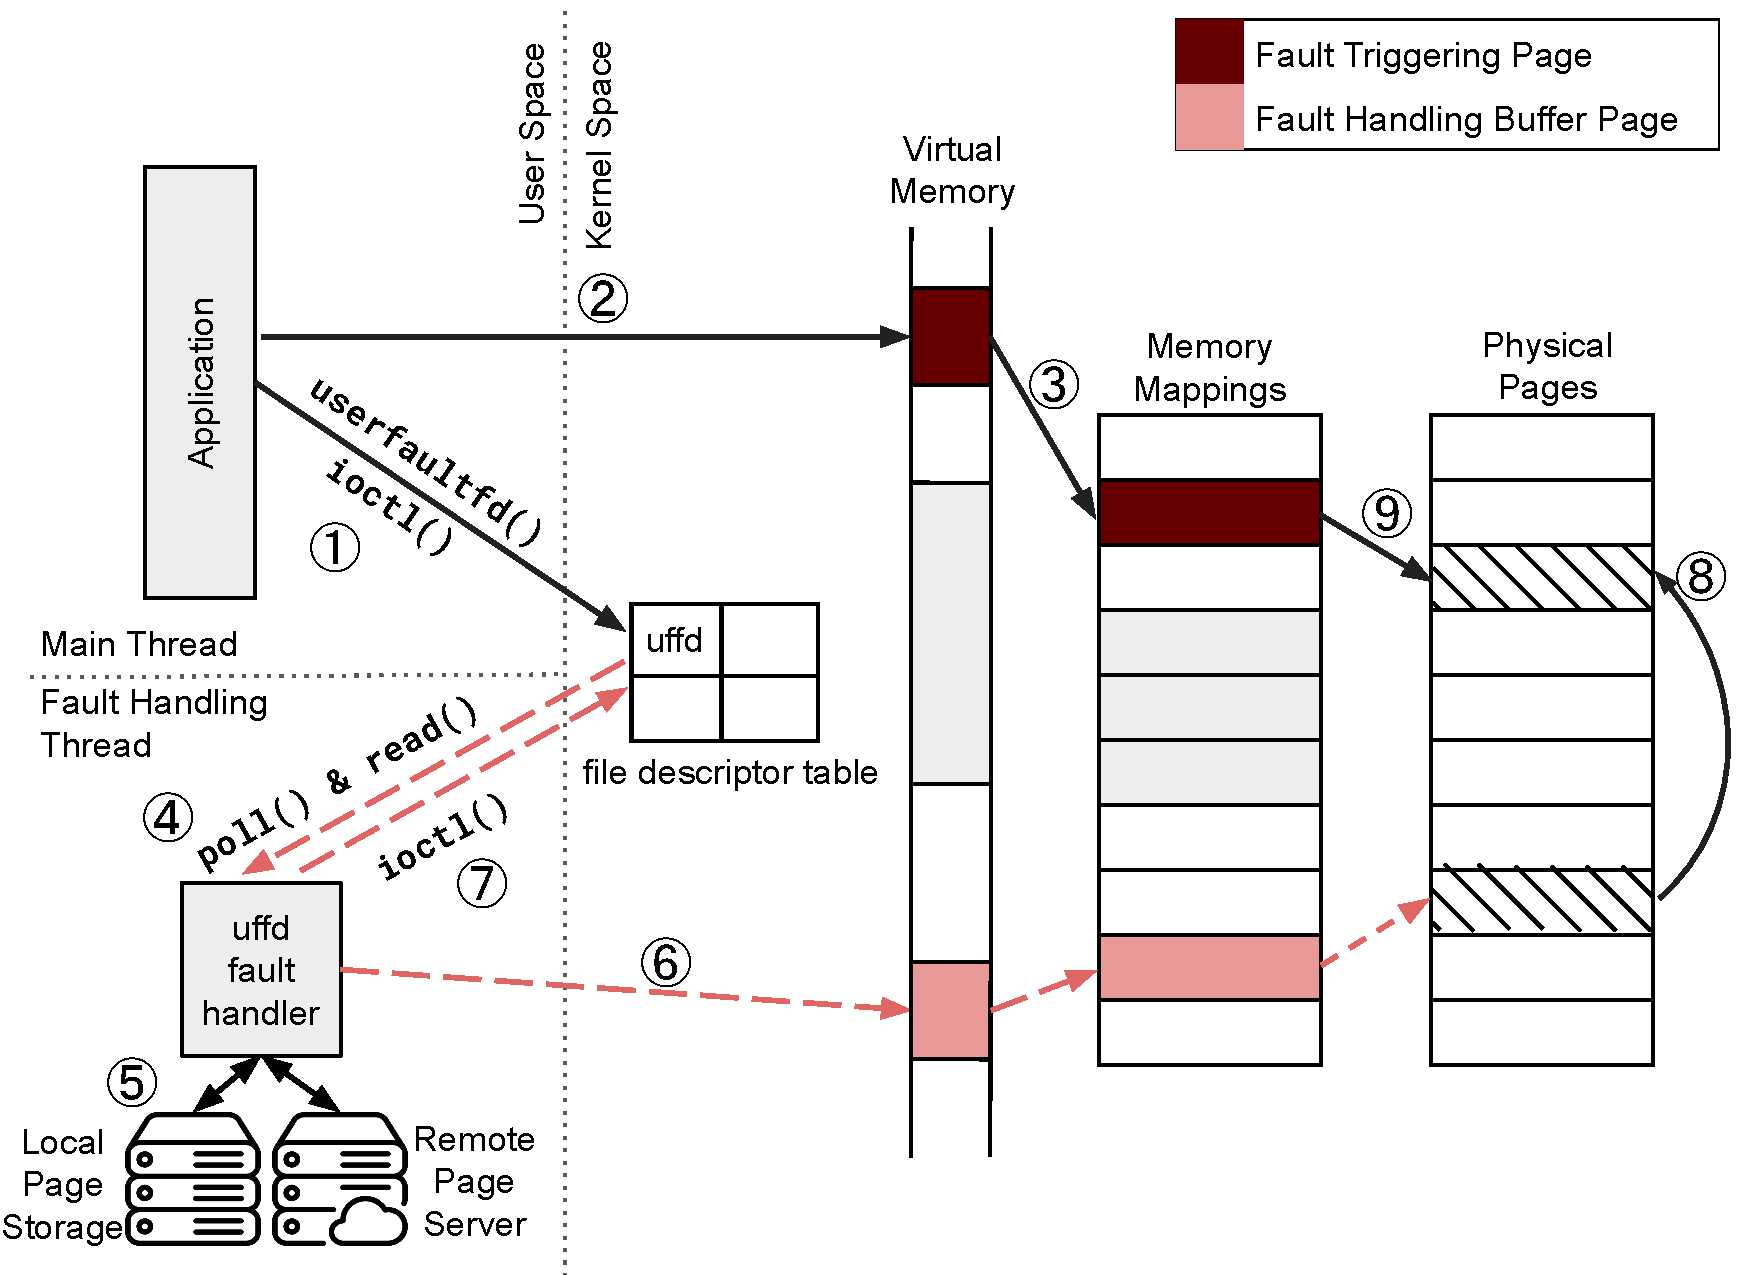
\includegraphics[clip,scale=0.26]{figures/uffd-v7.0.pdf}
    \caption{\texttt{userfaultfd()} workflow. }
    \label{fig:live-migration-diagram}
    %\vspace{-2em}
\end{figure}

% This corresponds to the "Local Page Storage" and "Remote Page Server"
Assuming we want to restore an application to a checkpointed state (\ie its state is stored on a local or remote disk), the CRIU client sets up an initial subset of the application's pages. The remaining pages aren't initialized yet, as we want to copy them the first time the application tries to access them, requiring a custom page fault handler. The CRIU client then calls \texttt{userfaultfd()}, creating a new uffd (userfault file descriptor), and uses \texttt{ioctl()} to register the regions of virtual memory (the application's remaining pages) it should handle (\pgftextcircled{1}). After creating a fault-handling thread that polls on the uffd, the application can safely resume execution.
When the application attempts to access an unmapped page (\pgftextcircled{2} and \pgftextcircled{3}), a page fault is raised. If the relevant page is in a \texttt{userfaultfd()}-registered region, the kernel marks the uffd as ready, waking up the fault-handling thread, which then reads from the uffd (\pgftextcircled{4}). For CRIU, the fault-handling thread will read the relevant data from the application's (local or remote) checkpoint (\pgftextcircled{5}) into a local buffer (\pgftextcircled{6}). The thread then submits a \texttt{userfaultfd()} command using \texttt{ioctl()} (\pgftextcircled{7}), which atomically copies the data into the application's address space, resolving the fault (\pgftextcircled{8}, \pgftextcircled{9}).

%Suppose we have an application we want to checkpoint. On the source side, we can either dump the memory to local disk or start a page server for the restored application to listen to requests of pages over the network, illustrated on the bottom left of Figure \ref{fig:live-migration-diagram}.
%On the restorer side,  we use \texttt{userfaultfd()} to create a new uffd (userfault file descriptor) and use the \texttt{ioctl()} system call with different flags to learn about available features and register one or more regions of virtual memory with certain kinds of page fault. At the same time, we create a fault-handling thread that polls on the uffds.

%Once a fault occurs in certain memory regions (\pgftextcircled{1} and \pgftextcircled{2} in Figure \ref{fig:live-migration-diagram}), the fault-handling thread will be woken up. It will either connect to the remote page server or read from local files to fill up a buffer page, then call \texttt{ioctl()} again with certain flags (usually \texttt{UFFDIO\_COPY}, which notify the fault triggering thread to copy (\pgftextcircled{4}) the buffer page to the faulting page (\pgftextcircled{5}, \pgftextcircled{6}, \pgftextcircled{7})). Finally, the application can access the content of the page ((\pgftextcircled{3}).

% \asaf{maybe guide this description (and also the rest of the paper) with an example of a specific application}

% Firecracker \cite{firecracker} provides a better management of the microVM's memory loading by letting users choose between relying on the host OS to handle the page faults when resuming from a snapshot, or having a dedicated userspace process for dealing with page faults, with the help of Userfaultfd.

%While \texttt{userfaultfd()} supports other modes, such as tracking minor faults and write-protected pages, we primarily focus on its major fault functionality.

In addition to CRIU, \texttt{userfaultfd()} has seen adoption in a number of large projects, along with more experimental work \cite{zIO, LightSwap, file-backed-article, file-backed-proceeding, uffd-security-framework-paper, TrailDB}. \texttt{userfaultfd()} is used by QEMU for VM post-copy migration, while Firecracker uses it to lazily restore microVM memory from a snapshot~\cite{firecracker}. The Android Runtime's garbage collector uses \texttt{userfaultfd()} in its compaction phase to track page accesses~\cite{Android_13_AOSP, garbage_collection_paper}.
Additionally, the authors of \texttt{userfaultfd()} have identified several additional potential use cases, such as distributed shared memory, language runtimes, and JIT compilers, along with adding support for handling write-protect and minor faults~\cite{LWN_Write-protect, LWN_next_step, LPC-presentation, uffd_presentation}.
Finally, we believe that there exist additional use cases for custom page fault handling which cannot utilize \texttt{userfaultfd()} due to its limitations, such as lazily resolving data relocations for position-independent executables in the dynamic linker, yielding faster program start-up~\cite{chromium-elf}.
We discuss these limitations in Section~\ref{sec:motivation}.

%A lot of other applications also benefit from the flexibility of customized page fault handling. Utilizing \texttt{userfaultfd()}, UMap\cite{file-backed-article, file-backed-proceeding} designs an interface akin to mmap but with faster access to large files. Lightswap \cite{LightSwap} enhances the performance of the swapping system. A lot of other work \cite{zIO, } also performs page fault interception. Some other user cases for memory observability.

\section{Limitations of Userspace Fault Handling}
\label{sec:motivation}

\texttt{userfaultfd()}'s design allows applications to fully customize page fault handling, with practically no limitations on the fault-handling routine. However, its design also incurs significant costs. In this section, we describe three limitations of \texttt{userfaultfd()}: scalability, applicability, and security.

\textbf{Scalability.}
In multi-threaded applications, typically each thread's page faults are handled in-kernel by the respective thread. However, for applications using \texttt{userfaultfd()}, there is only one fault-handling thread, which can become a performance bottleneck. To illustrate this, we run an experiment with and without \texttt{userfaultfd()}: we set up a pool of threads, each of which is allocated 50 pages of anonymous memory, and access each of those pages, generating 50 page faults per thread. We then fill each page with a fixed value, either in the handling routine (using \texttt{userfaultfd()}) or in the thread loop (default fault handling). As shown in Figure~\ref{fig:motivation-scalability}, as the number of threads increases, \texttt{userfaultfd()} takes significantly longer to handle page faults and scales worse than the standard kernel handling.

%\asaf{maybe it's worth motivating very briefly why running so many threads would be a realistic scenario in applications that would use userfaultfd} \teng{high-traffic web/db servers or hpc?}

% We demonstrate this effect by running a microbenchmark: we \texttt{mmap()} 50 pages of anonymous memory for each thread, register them with \texttt{userfaultfd()} and pass the uffd to the fault handling thread. Each thread triggers page faults by performing memory access to each page concurrently. For simplicity, the buffer page is \texttt{memset()}'ed with random values. For each setting, we take an average of 50 runs. \tal{add experiment description}. As shown in Figure~\ref{fig:motivation-scalability}, as the number of threads increases, \texttt{userfaultfd()} takes significantly longer to handle page faults and scales much worse than the standard kernel handling.

%To illustrate this effect, we conducted a microbenchmark experiment by creating a pool of threads - each thread mapped 50 pages of anonymous memory using \texttt{mmap()}, registered these pages with \texttt{userfaultfd()}, and passed the fd to the fault-handling thread. Each thread triggered page faults by accessing each page concurrently. For simplicity, the handler filled buffer pages with random values using \texttt{memset()}. We repeated this process for 50 runs and calculated the average time taken for each different number of threads in the pool. 

Additionally, each \texttt{userfaultfd()} fault-handling routine requires at least three syscall invocations: \texttt{poll()}, \texttt{read()}, and \texttt{ioctl()}. Each of these syscalls requires user-kernel crossings, which add overhead for each page fault, in addition to the cost of context switching to the fault-handling thread. Finally, \texttt{userfaultfd()}'s design may lead to unnecessarily copying data between userspace and kernel space. For example, in the VM migration use case, data read from the network is copied to userspace through \texttt{recv()}, and then copied back to the kernel as part of the \texttt{userfaultfd()} resolution code. Since the data is already present in the kernel, this overhead is unnecessary.


\begin{figure}[h]
    \centering
    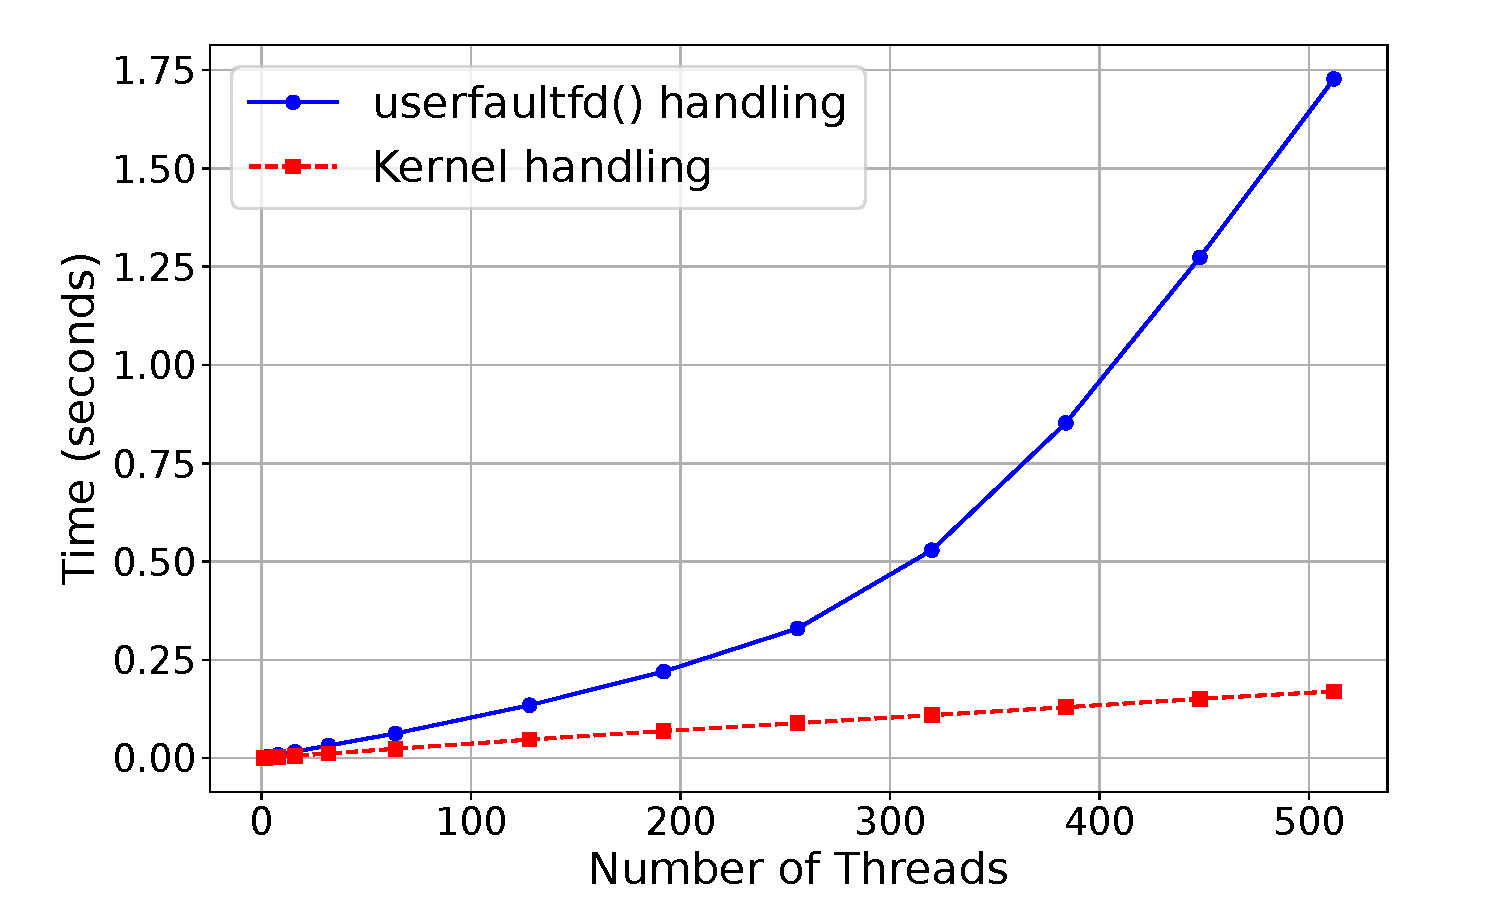
\includegraphics[clip,scale=0.33]{figures/uffd-scalability-motivation.pdf}
    %\vspace{-0.5em}
    \caption{Latency to handle 50 page faults per thread.}
    \label{fig:motivation-scalability}
    %\vspace{-1.0em}
\end{figure}

\textbf{Applicability.} The use of a dedicated fault-handling thread limits which systems can use \texttt{userfaultfd()}.
Specifically, applications that fork may not be able to use \texttt{userfaultfd()}, as forking in a multi-threaded environment only clones the thread that calls \texttt{fork()}, potentially leading to incorrect behavior.
This effectively prevents \texttt{userfaultfd()} from being used in interchangeable libraries, such as the dynamic linker or garbage collectors, which cannot restrict application behavior in such a way.

\textbf{Security.} \texttt{userfaultfd()} has been used in a number of kernel exploits~\cite{uffd-blocking,dirtycred,linux-heap-cve,linux-heap-spray,linux-uaf-cve}, many of which have taken advantage of its ability to indefinitely block kernel execution at a specific point. While mitigations have been proposed and merged~\cite{uffd-blocking}, container runtimes such as Docker have blocked its usage in their default configurations due to these security concerns~\cite{docker-seccomp}, further limiting its applicability.
\section{Design}
\label{sec:design}

% \begin{figure}[]
%     \centering
%     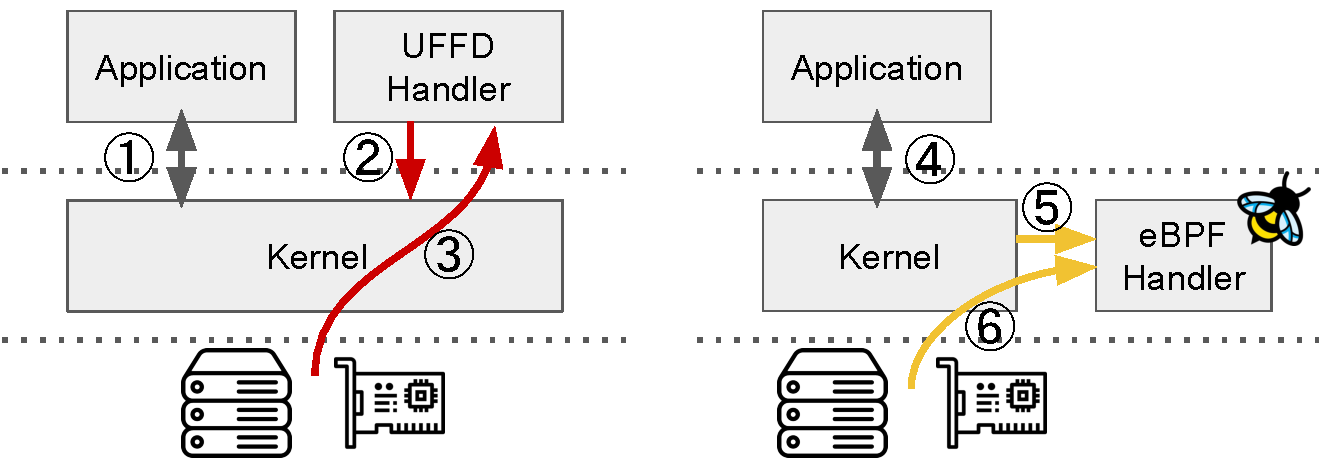
\includegraphics[clip,scale=0.33]{figures/Comparison.pdf}
%     \vspace{-0.5em}
%     \caption{When application triggers page faults (\pgftextcircled{1}, \pgftextcircled{4}), Kernel wakes up uffd handler (\pgftextcircled{2}) or calls eBPF handler (\pgftextcircled{5}). Handler fetches source pages (3, 6), processes them, and returns to kernel. Compared with \pgftextcircled{5} \& \pgftextcircled{6}, \pgftextcircled{2} \& \pgftextcircled{3} incurs overhead with kernel crossing.}
%     \label{fig:motivation-scalability}
%     \vspace{-1.0em}
% \end{figure}

In order to mitigate some of the downsides of \texttt{userfaultfd()}, we propose an \textbf{eBPF-based system} to register custom page fault handlers in-kernel.
%While \texttt{userfaultfd()} has a few different modes of operation, we initially focus on replicating its missing pages functionality.
This system requires two key modifications to the kernel, which we describe in this section.

% Figure xxx is the overall design of our eBPF-powered page fault-handling routine.

\textbf{Per-VMA eBPF programs}. Each eBPF fault-handling program must be associated with a range of the process's address space. The relevant kernel data structure is the \texttt{struct vm\_area\_struct}, which represents a contiguous virtual memory area (VMA). As such, we add support for per-VMA eBPF programs, similar to the kernel's support for per-cgroup eBPF programs~\cite{per-cgroup-bpf}.
After loading and verifying the eBPF program, the application attaches it to a specific address range. The kernel then translates that address range to a VMA (or series of VMAs), and associates the eBPF program with those VMAs.
If the address range starts or ends within a VMA, the kernel will split the VMA, as is done with \texttt{userfaultfd()}.

\textbf{Fault-handling modifications.} We modify the kernel's page fault-handling routine to check if an eBPF program is attached to the relevant VMA. If so, we run the eBPF program, providing metadata about the fault, along with access to a newly allocated page to fill with the desired contents. After the eBPF program executes, we resolve the fault by setting the relevant memory mappings to point to the new page. This removes the need for an additional memory copy, as is done in \texttt{userfaultfd()}, which fills the page in userspace and then copies it into the kernel. We envision this design enabling zero-copy page faults, with data read from the disk or network written directly to the relevant page.

For simple fault-handling routines, the aforementioned kernel changes should be sufficient. However, for more complex applications such as VM migration which require reading data from the network or disk, we envision adding eBPF helpers to support such operations, along with building on the existing support for sleepable eBPF programs~\cite{sleepable-bpf}.

We believe that this implementation removes the need for an additional fault-handling thread and reduces unnecessary kernel crossings or data copying. While eBPF may somewhat limit the flexibility of the custom fault handlers, we believe that eBPF is mature enough to handle interesting and complex use cases. Additionally, the eBPF verifier could be used to limit the operations used in the handling routine, such as sleeping indefinitely, potentially addressing the security concerns that plague \texttt{userfaultfd()}.


\section{Acknowledgments}
This work was supported by Intel and IBM, and NSF awards CNS-2143868 and CNS-2104292.
Tal Zussman was supported by NSF award DGE-2036197.


\label{lastpage}

\bibliographystyle{ACM-Reference-Format}
\bibliography{reference}

\end{document}